\documentclass[10pt,a4paper,twocolumn]{article}

\usepackage[cm]{fullpage}
\usepackage{caption}
\usepackage{subcaption}
\usepackage{hyperref}
\usepackage{newtxtext}
\usepackage{newtxmath}
\usepackage{listings}
\usepackage{graphicx}
\usepackage{color}
\usepackage{titlesec}
\usepackage{subcaption}

% \let\oldv\verbatim
% \let\oldendv\endverbatim

% \def\verbatim{\par\setbox0\vbox\bgroup\oldv}
% \def\endverbatim{\oldendv\egroup\fboxsep0pt \noindent\colorbox[gray]{0.8}{\usebox0}\par}

\newcommand{\cmmnt}[1]{}

\definecolor{verbgray}{gray}{0.9}

\lstnewenvironment{code}{%
  \lstset{backgroundcolor=\color{verbgray},
  frame=single,
  framerule=0pt,
  basicstyle=\ttfamily,
  columns=fullflexible}}{}

% \definecolor{shadecolor}{rgb}{.9, .9, .9}

\setlength\parindent{0pt}
\setlength{\parskip}{5pt}
\titlespacing\section{0pt}{12pt plus 4pt minus 2pt}{0pt plus 2pt minus 2pt}
\titlespacing\subsection{0pt}{12pt plus 4pt minus 2pt}{0pt plus 2pt minus 2pt}
\titlespacing\subsubsection{0pt}{12pt plus 4pt minus 2pt}{0pt plus 2pt minus 2pt}


\title{Conversational Interfaces (M)\\Assessed Coursework Report}
\author{Inesh Bose}
\date{}

\begin{document}

\maketitle

\section*{Abstract}

Football Agent is a conversational chatbot developed for the COMPSCI5094 Conversational Interfaces (M) coursework, during the academic session 2022-2023, that interacts with API-Football to provide users with information based on questions around the football domain. The base version was developed with Alexa, but the implementation has been extended to be modular, providing a separate package to integrate with the API using only the info-type that an utterance is expecting, and to demonstrate that, the agent was also built using Wit.ai and deployed on a static generated website for demonstration.

\section{Introduction}

This coursework required the development of a task-oriented dialogue system, using a conversational toolkit (such as Rasa, Dialogflow and Wit.ai), that lets a user access various information about football teams in the English Premier League.

A set of sample dialogues in the football information domain was provided. These were used to gather the idea \& expectations and to infer intents, slots, and utterances. Furthermore, unseen dialogues would be provided later in the development to evaluate the NLU component. The adviced API was \href{https://www.api-football.com/}{API-Football} \cite{APIFootb40:online}.

\section{Part A}

The first part of this coursework aimed to develop \& build the conversational agent based on the sample dialogues allowing the user to know information about the football teams based on input (intent); then its NLU performance would be evaluated using the test dialogues without needing to alter the implementation.

\subsection{Agent Development \cmmnt{\small (6 marks)}}

The toolkit chosen for this coursework was \href{https://developer.amazon.com/en-GB/alexa}{\textbf{Alexa}} \cite{AmazonAl18:online} with the skill developed in \href{https://nodejs.dev/}{\textbf{Node.js}} \cite{RunJavaS19:online} - but not in \href{https://nodejs.org/docs/latest/api/modules.html}{CommonJS} \cite{ModulesC3:online} and not in the small dashboard that Amazon provides. So, the code would be written in \href{https://typescriptlang.org/}{TypeScript} \cite{TypeScri1:online} enabling the usage of \href{https://nodejs.org/docs/latest/api/esm.html}{ES Modules} \cite{ModulesE42:online} and more importantly, type safety. The code would be transpiled into the required format on the fly using \href{https://github.com/unjs/jiti}{\texttt{jiti}} \cite{GitHubun42:online}. This enabled development to be incredibly less painful and less time-consuming (with the argument of setup trade-off); there is also \href{https://marketplace.visualstudio.com/items?itemName=ask-toolkit.alexa-skills-kit-toolkit}{an extension} for Visual Studio Code to test and debug Alexa Skills, so the bot could be run locally \cite{AlexaSki43:online}. \href{https://git-scm.com/}{Git} \cite{Git14:online} was also used for version control and deploying to AWS Lambda.

Based on the sample dialogues, there is one intent \texttt{GetInfo} that would have slots \texttt{team}, that is required, and \texttt{info}. Some examples included multiple values for \texttt{info} while the assistant only responds using one (the first) - allowing multiple would be an extension. Moreover, while \texttt{team} is required, \texttt{info} can be empty and in that case, it can be assumed to be \texttt{leaguePosition}. Session attributes would be used to allow \texttt{team} to be inferred from words like \texttt{"they"} and \texttt{"their"}. The teams can be assumed to be from the Premier League roster and in the season "2022" (since the year has been completed with reliable data from the API). Some difficulties would be inferring the \texttt{info} value based on the sentence or picking keywords \textit{around} the \texttt{team}s - a workaround may have been having more, separate slots or have them as intents but the sample dialogues did not use the format therefore this configuration was set with specific keywords linking to each \texttt{info} type (such as \texttt{"record"} for \texttt{winLossRecord}, \texttt{"playing right now"} for \texttt{playingNow} and \texttt{"manager"} for \texttt{manager}) which could mean that if user input doesn't make grammatical sense (like \texttt{"\textit{who} is Arsenal's record"}), it would still answer (as \texttt{"what"}).

\begin{figure}[h]
    \centering
    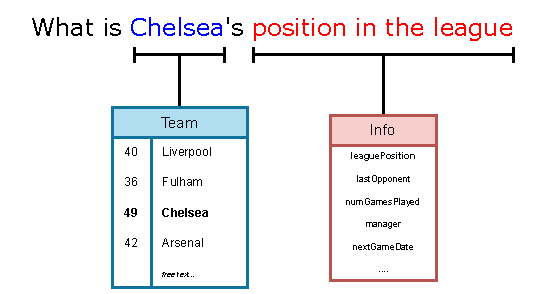
\includegraphics[width=0.45\textwidth]{assets/utterance-example.pdf}
    \caption*{Example breakdown of utterance}
\end{figure}

Moreover, slots were assigned synonyms; while it was not required for \texttt{team} (like \texttt{Wolverhampton Wanderers} as \texttt{wolves}), it was essential for \texttt{info}. The values also had \texttt{id} assigned; this is optional too, but it was very helpful for quicker parsing. The system handles scenarios where \texttt{id} is not provided.

The type definitions for clarity can be seen in \href{https://github.com/ineshbose/UofG_Conversational_Interfaces/blob/master/packages/api/types.ts}{\texttt{types.ts}} along with a linker for API-endpoint to \texttt{info} type in \href{https://github.com/ineshbose/UofG_Conversational_Interfaces/blob/master/packages/api/intent/linker.ts}{\texttt{linker.ts}} in the code repository on \href{https://github.com/ineshbose/UofG_Conversational_Interfaces}{https://github.com/ineshbose/UofG\_Conversational\_Interfaces}.

\begin{figure}[h]
    \vspace{1cm}
    \centering
    \begin{code}
  User: open football agent
  Assistant: How can I help?

  User: What is Chelsea's position in the league
  Assistant: Chelsea are in 10th place
    in the Premier League standings.

  User: What is their record so far?
  Assistant: Chelsea have 10 wins, 9 loses and
    8 draws in the Premier League standings.

  User: Are they playing right now?
  Assistant: No.

  User: Who is their manager?
  Assistant: The manager/coach for Chelsea
    is E. Hayes
    \end{code}
    \caption*{Sample dialogue with the agent}
    \vspace{1cm}
\end{figure}

\begin{figure}[h!]
    \captionsetup{labelformat=empty}
    \centering
    \begin{subfigure}[b]{0.24\textwidth}
        \centering
        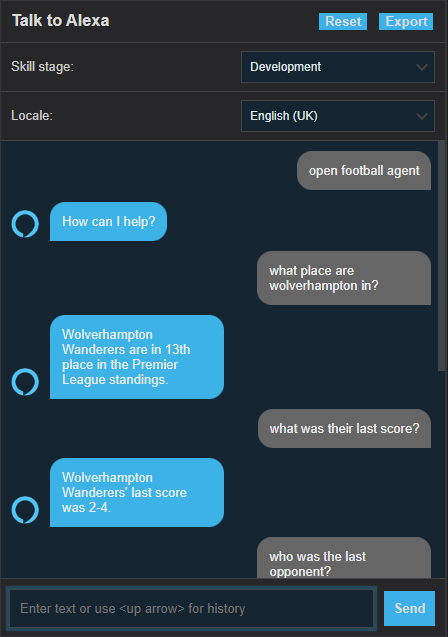
\includegraphics[width=\textwidth]{assets/Screenshot_1.png}
    \end{subfigure}
    \hfill
    \begin{subfigure}[b]{0.24\textwidth}
        \centering
        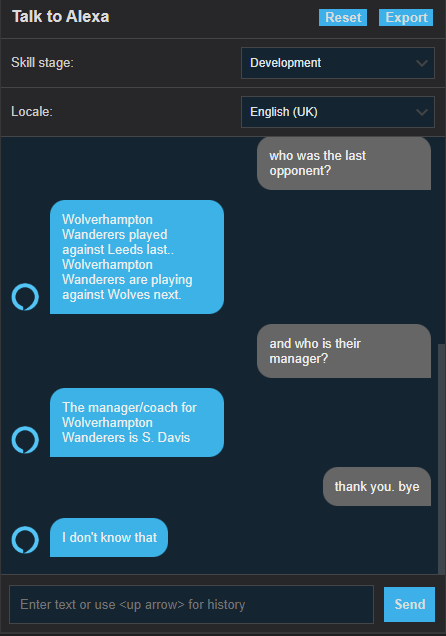
\includegraphics[width=\textwidth]{assets/Screenshot_2.png}
    \end{subfigure}
    \vskip\baselineskip
    \begin{subfigure}[b]{0.24\textwidth}
        \centering
        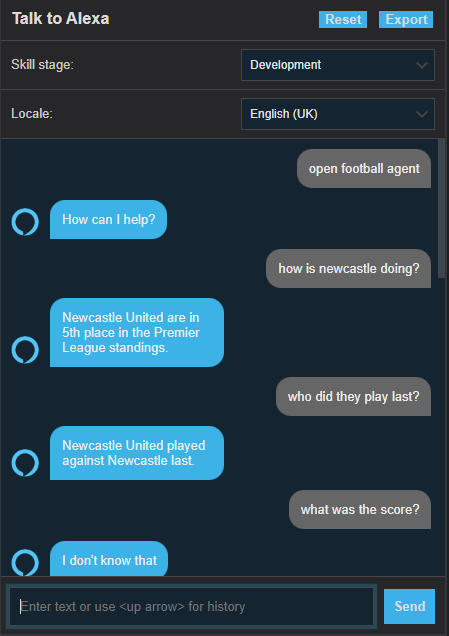
\includegraphics[width=\textwidth]{assets/Screenshot_3.png}
    \end{subfigure}
    \hfill
    \begin{subfigure}[b]{0.24\textwidth}
        \centering
        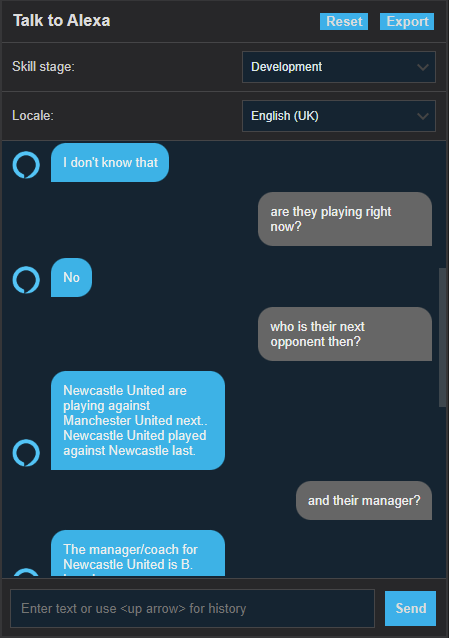
\includegraphics[width=\textwidth]{assets/Screenshot_4.png}
    \end{subfigure}
    \caption*{Conversation with the Alexa Skill bot}
    \vspace{0.5cm}
\end{figure}

\subsection{NLU Evaluation \cmmnt{\small (5 marks)}}

Using the provided instructions and examples, the NLU effectiveness was evaluated turn-by-turn on the 13 test dialogues.

\begin{itemize}
    \setlength\itemsep{0em}
    \item \textbf{TP}: \textit{True Positive} - intent and slots are expected from the statement, and the system correctly detects it
    \item \textbf{TN}: \textit{True Negative} - intent and slots are not expected from the statement so the system doesn't detect it (not measured)
    \item \textbf{FP}: \textit{False Positive} - intent and slots are not expected from the statement but the system somehow detects it
    \item \textbf{FN}: \textit{False Negative} - intent and slots are expected from the statement but the system doesn't detect it in the utterance
\end{itemize}

\begin{table}[h]
\centering
\begin{tabular}{lllll}
\hline
name           & TP & TN & FP & FN \\ \hline
GetInfo        & 61 & 0  & 0  & 1  \\
Team           & 61 & 0  & 0  & 1  \\
lastOpponent   & 5  & 0  & 0  & 2  \\
lastScore      & 2  & 0  & 0  & 9  \\
leaguePosition & 9  & 1  & 0  & 3  \\
manager        & 11 & 0  & 0  & 2  \\
nextGameDate   & 1  & 0  & 0  & 2  \\
nextOpponent   & 3  & 0  & 1  & 0  \\
numGamesPlayed & 4  & 0  & 1  & 2  \\
playingNow     & 5  & 0  & 2  & 0  \\
winLossRecord  & 1  & 0  & 1  & 1  \\ \hline
\end{tabular}
\caption*{Final table for NLU evaluation}
\end{table}

Based on the above values for each dialogue, the Precision, Recall and F1 would be calculated using the following formula:

\begin{itemize}
    \setlength\itemsep{0em}
    \item \textbf{Precision ($P$)}: $TP \div (TP + FP)$
    \item \textbf{Recall ($R$)}: $TP \div (TP + FN)$
    \item \textbf{F1}: $(2 * P * R) \div (P + R)$
\end{itemize}

\begin{table}[h]
\centering
\begin{tabular}{llll}
\hline
name           & Precision & Recall & F1     \\ \hline
GetInfo        & 1.0       & 0.98   & 0.99   \\
Team           & 1.0       & 0.9839 & 0.9919 \\
lastOpponent   & 1.0       & 0.7143 & 0.8333 \\
lastScore      & 1.0       & 0.1818 & 0.3077 \\
leaguePosition & 1.0       & 0.75   & 0.8571 \\
manager        & 1.0       & 0.8462 & 0.9167 \\
nextGameDate   & 1.0       & 0.3333 & 0.5    \\
nextOpponent   & 0.75      & 1.0    & 0.8571 \\
numGamesPlayed & 0.8       & 0.6667 & 0.7273 \\
playingNow     & 0.7143    & 1.0    & 0.8333 \\
winLossRecord  & 0.5       & 0.5    & 0.5    \\ \hline
\end{tabular}
\caption*{Metrics of the agent}
\end{table}

The results for the agent are good for the initial version (and there is room for improvement). All data for evaluation can be found in the \href{https://github.com/ineshbose/UofG_Conversational_Interfaces/blob/master/docs/test-data}{\texttt{/docs/test-data}} directory in the repository.

\section{Part B}

The second part of this coursework aimed to extend the agent (and optionally implement it). Being very passionate and interested in making modular Node.js packages and web technology enabled proficient development in extending the agent.

\subsection{Extended Design \cmmnt{\small (5 marks)}}

The aim is to provide a live demonstration of the agent outside of the restrictive platform allowing the system to be easily accessible over a simple website link without many resources, and additionally enable it to be toolkit-agnostic (not be specific to one platform service) so it should be easily usable and deployed with other toolkits of preference. Moreover, it would be much better if the bot responds faster to the user (improving user experience) than having them wait while the backend makes the API calls. Additionally, some provided examples used multiple values for the \texttt{info} slot - so it also be very useful for the bot to respond to every type of information a user is asking for.

\begin{figure}[h]
    \centering
    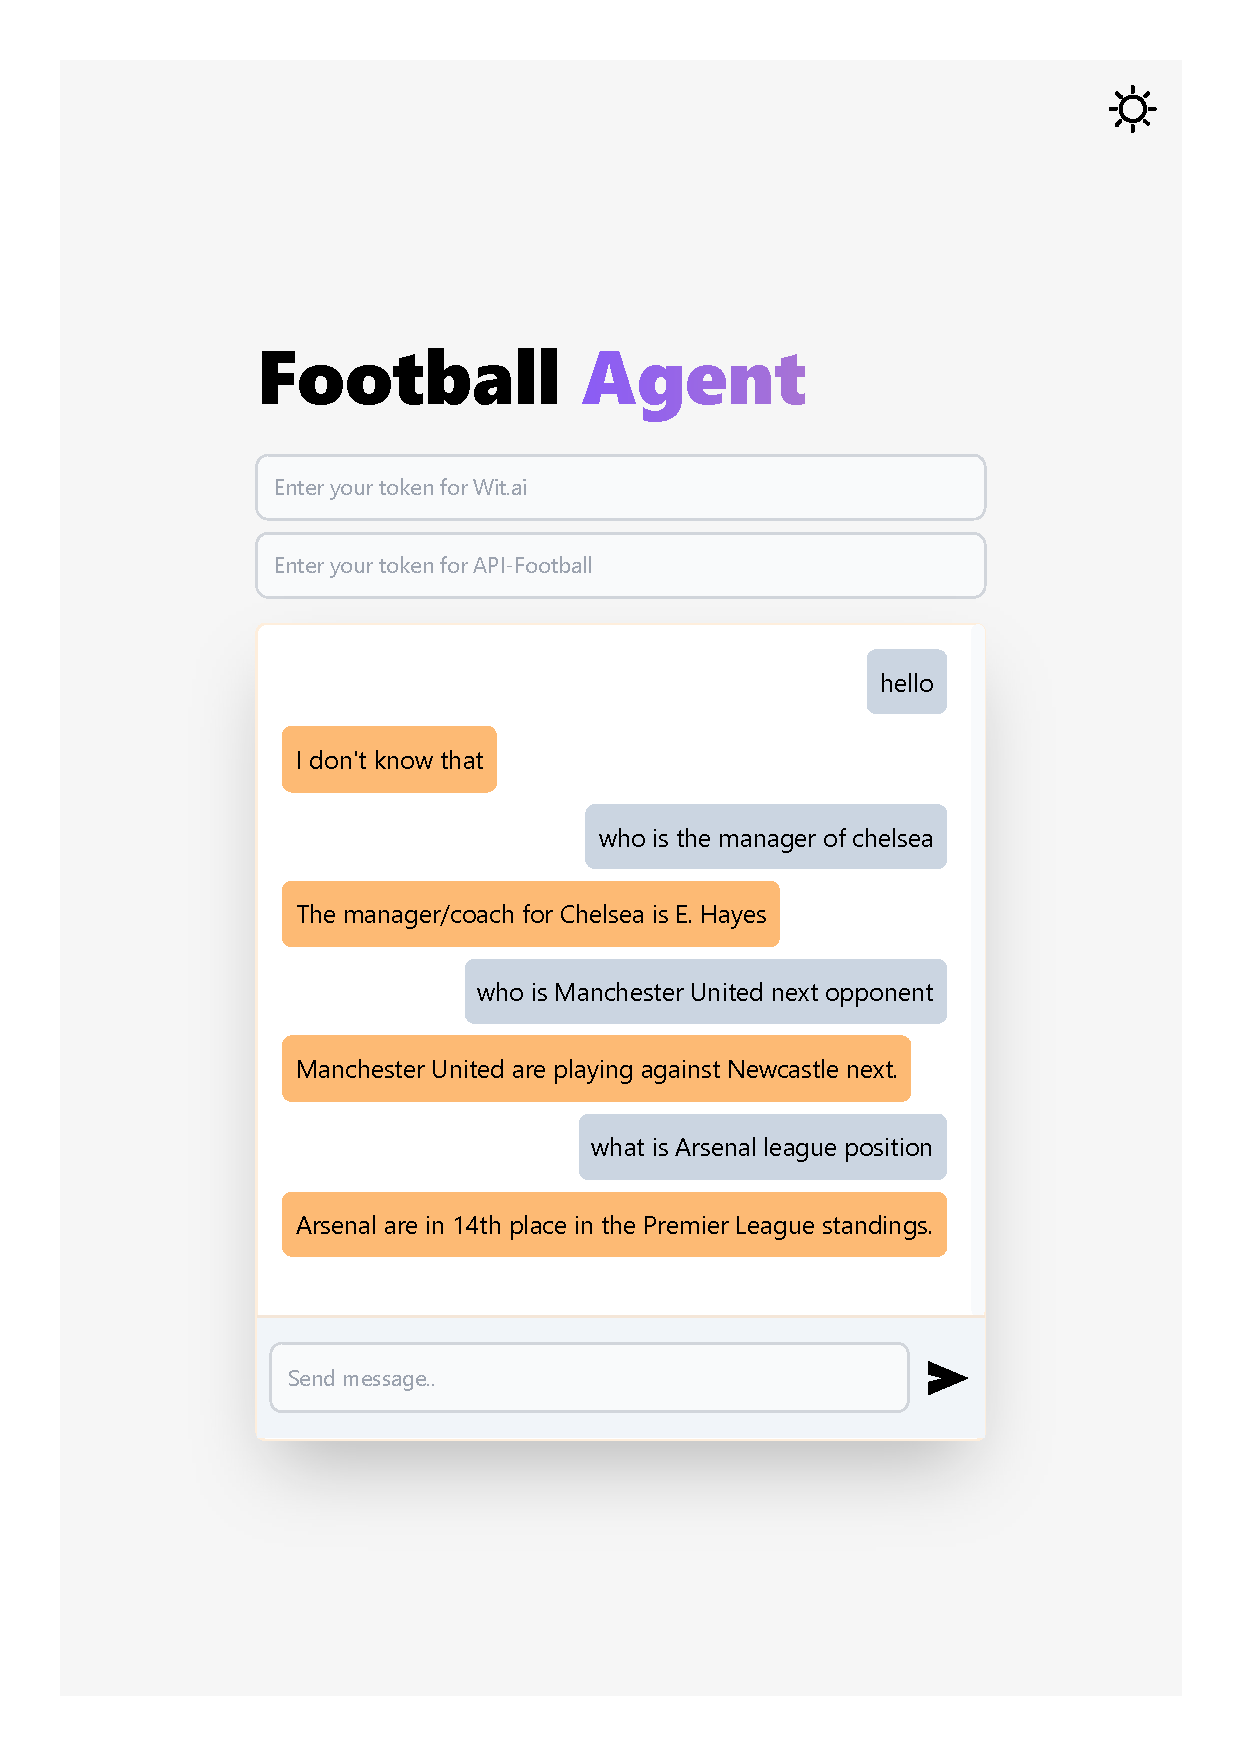
\includegraphics[width=0.4\textwidth]{assets/ui-preview.pdf}
    \caption*{UI Design of the Planned Deployed Demo}
\end{figure}

Alexa does not provide a clear HTTP REST API to interact with (only Alexa-enabled devices from Amazon onto ARN Lambda Endpoints), so another toolkit may need to be chosen. Dialogflow provides integration to platforms such as Twilio and Facebook Messenger, but not with a self-hosted website to accept HTTP requests from. Ideally, progress should not be discarded either. The process could pose to be time-consuming and not very effective; it could limit agents from fully utilising all functionality that a toolkit provides. Caching responses may also cause incorrect, outdated information to be stored. Moreover, APIs require authorisation tokens and those cannot be openly provided unless a server could be set up which would require funding. Therefore, a lot of designs and planning would be required in the initial stage to implement with confidence.

\begin{figure*}
    \centering
    \begin{subfigure}[b]{0.48\textwidth}
        \centering
        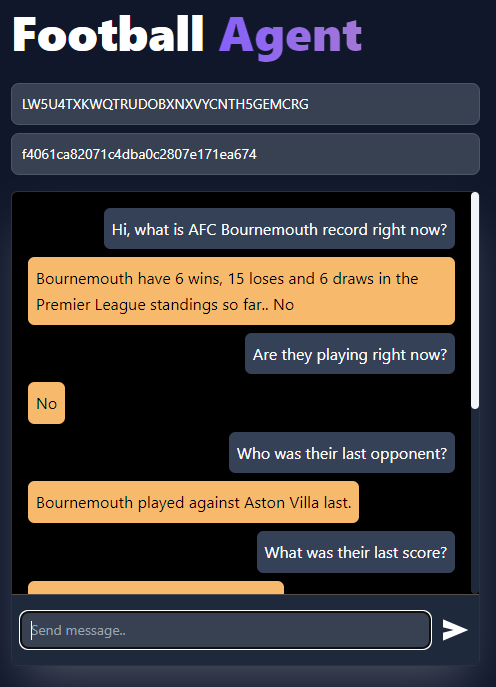
\includegraphics[width=\textwidth]{assets/Screenshot_5.png}
    \end{subfigure}
    \hfill
    \begin{subfigure}[b]{0.47\textwidth}
        \centering
        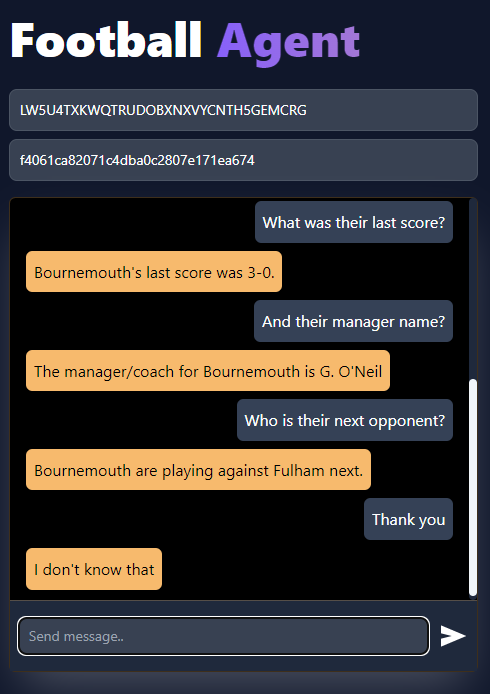
\includegraphics[width=\textwidth]{assets/Screenshot_6.png}
    \end{subfigure}
    \caption*{Conversation 1 with the demo app}
\end{figure*}

\begin{figure*}
    \centering
    \begin{subfigure}[b]{0.48\textwidth}
        \centering
        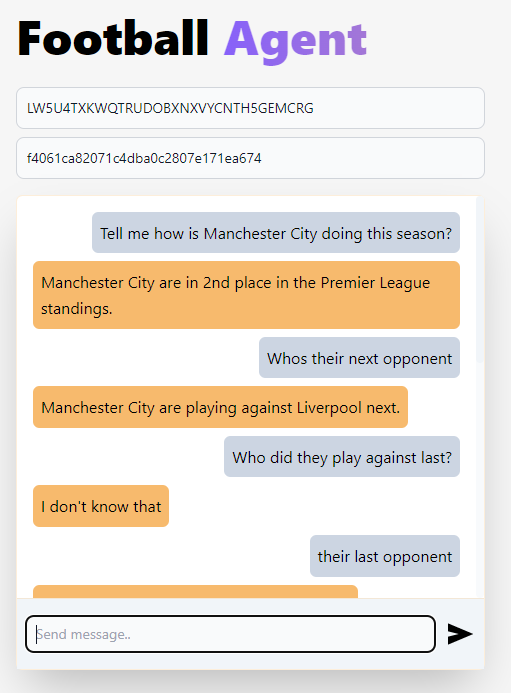
\includegraphics[width=\textwidth]{assets/Screenshot_9.png}
    \end{subfigure}
    \hfill
    \begin{subfigure}[b]{0.48\textwidth}
        \centering
        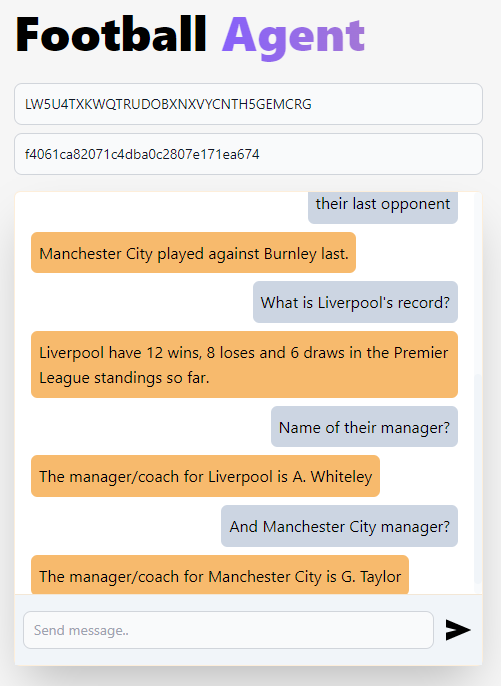
\includegraphics[width=\textwidth]{assets/Screenshot_10.png}
    \end{subfigure}
    \caption*{Conversation 2 with the demo app}
\end{figure*}

\begin{figure*}
    \centering
    \begin{subfigure}[b]{0.4772\textwidth}
        \centering
        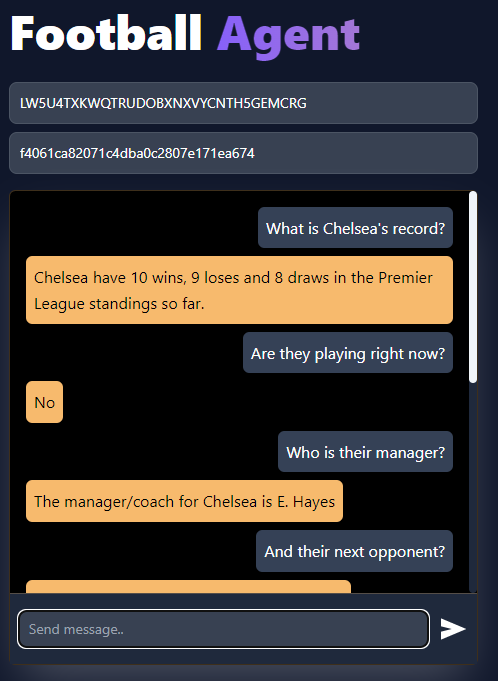
\includegraphics[width=\textwidth]{assets/Screenshot_7.png}
    \end{subfigure}
    \hfill
    \begin{subfigure}[b]{0.48\textwidth}
        \centering
        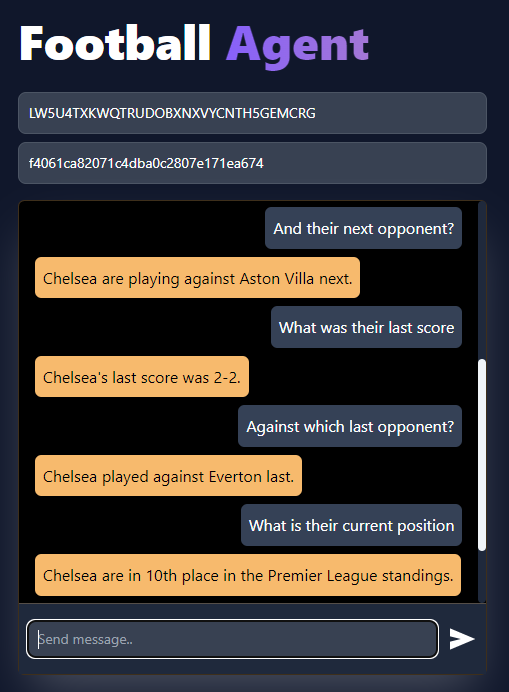
\includegraphics[width=\textwidth]{assets/Screenshot_8.png}
    \end{subfigure}
    \caption*{Conversation 3 with the demo app}
\end{figure*}

\begin{figure*}
    \centering
    \begin{subfigure}[b]{0.48\textwidth}
        \centering
        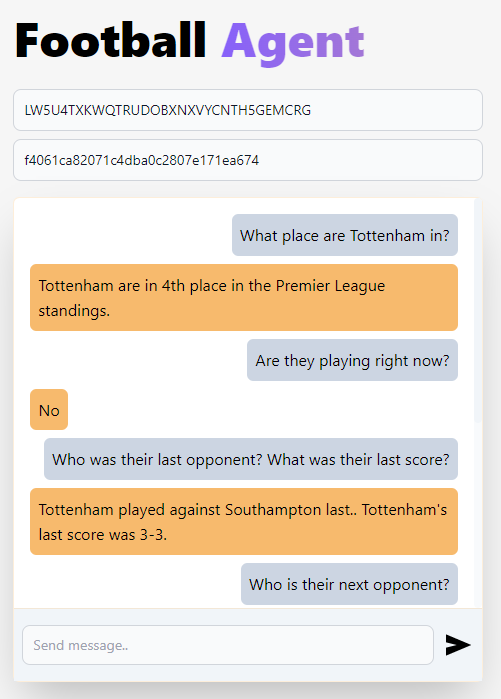
\includegraphics[width=\textwidth]{assets/Screenshot_11.png}
    \end{subfigure}
    \hfill
    \begin{subfigure}[b]{0.48\textwidth}
        \centering
        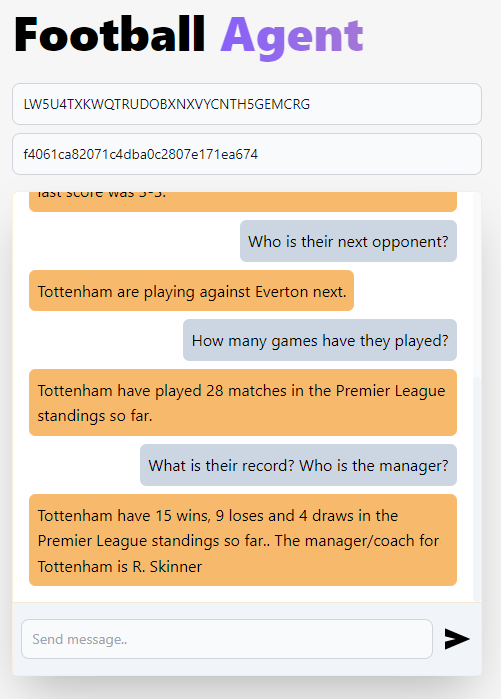
\includegraphics[width=\textwidth]{assets/Screenshot_12.png}
    \end{subfigure}
    \caption*{Conversation 4 with the demo app}
\end{figure*}

\begin{figure*}
    \centering
    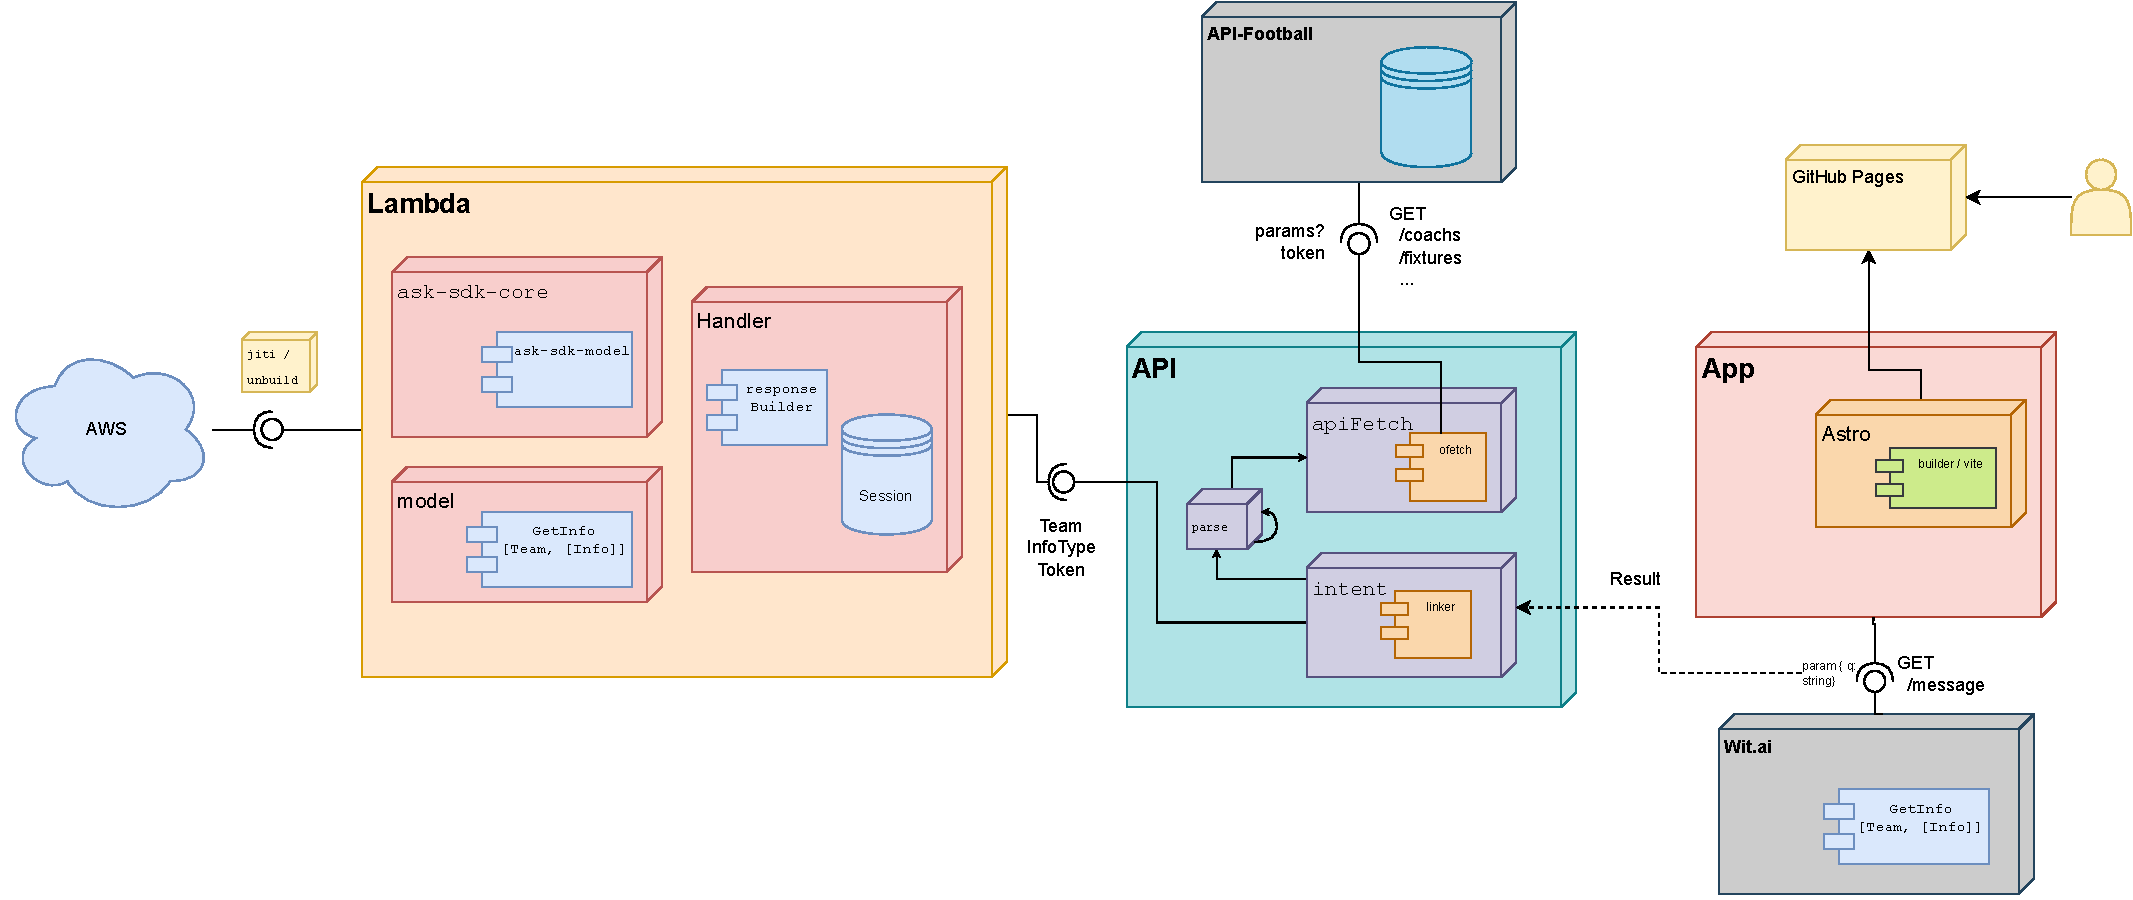
\includegraphics[width=\textwidth]{assets/architecture.pdf}
    \caption*{System Architecture}
\end{figure*}

\begin{figure*}
    \centering
    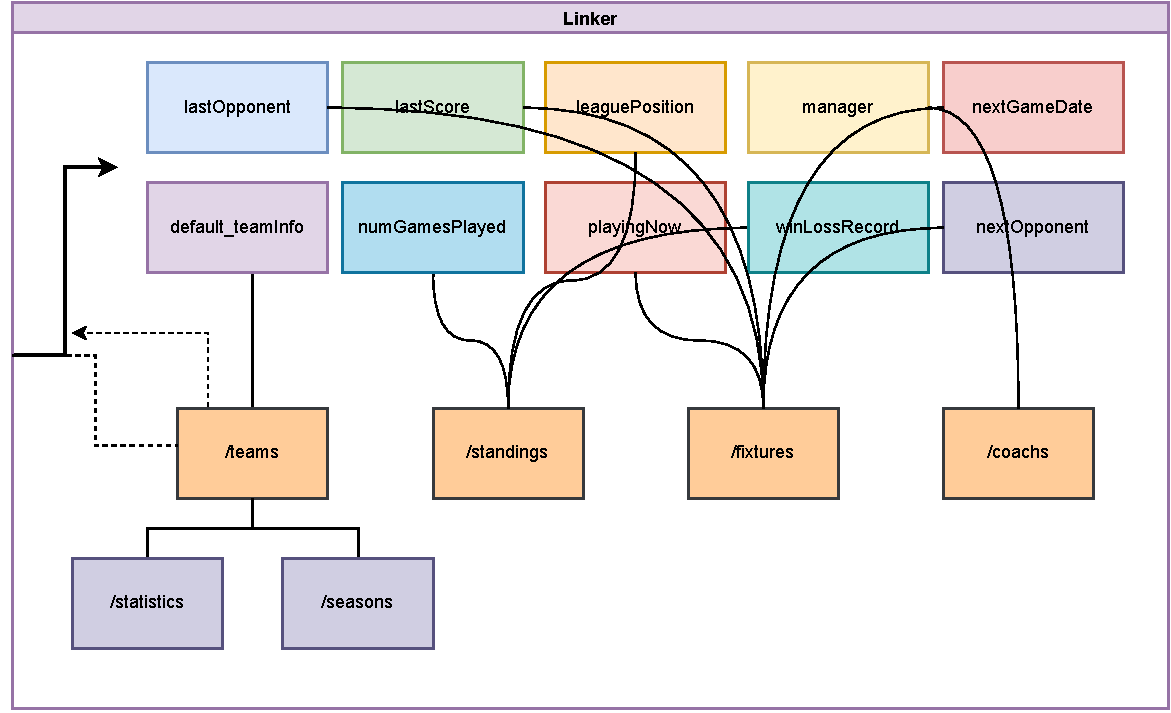
\includegraphics[width=0.8\textwidth]{assets/linker.pdf}
    \caption*{Mapping of \texttt{info} type to endpoint}
\end{figure*}

\subsection{Extended Implementation \cmmnt{\small (6 marks)}}

The implementation would be done in a monolithic repository with three packages - \texttt{lambda} (for Alexa), \texttt{api} (for parsing and API interaction), and \texttt{app} (which would include the demo).

The \texttt{api} package provides a function \texttt{getInfo} that takes in the slots and returns a string message as a response. Internally, the function would iterate over \texttt{info}, calling the API to each endpoint linked to \texttt{info} type using a switch statement in \texttt{linker.ts}. The responses would be cached in a variable that uses the endpoint and query parameters to identify a value (also helping in staying under the API-Football usage limit). To solve the REST API problem, Wit.ai provides a \texttt{/message} endpoint with excellent documentation \cite{Witai58:online}, so the implementation was able to make use of that. The site was generated using Astro \cite{Astro7:online} and minimum dependencies, so it is highly performant \& accessible being deployed on GitHub Pages for free.

The demo is on \href{https://inesh.xyz/UofG_Conversational_Interfaces/}{https://inesh.xyz/UofG\_Conversational\_Interfaces/} with tokens \texttt{[removed]} and \texttt{[removed]} for Wit.ai and API-Football\footnote{ensuring access is not suspended, otherwise please feel free to email} respectively. The application source-code is also available on the repository in the \texttt{packages/app} directory.

\bibliographystyle{plain}
\footnotesize{\bibliography{references}}

\end{document}
